% !TEX root = master_thesis.tex
\chapter{Discussion of results}
This chapter will present a discussion of results for the beam asymmetry $\Sigma$ in the reaction $\gamma p \to p\eta'\to p\gamma\gamma$ obtained with the CBELSA/TAPS experiment. No dedicated discussion of the results obtained for $\eta$ photoproduction will be given here. Very good agreement between the results for $\Sigma_\eta$ in this work and reference \cite{farahphd} makes this obsolete, because the findings for $\Sigma_\eta$ compared to various previous measurements and existing PWA predictions are discussed in reference \cite{farahphd} in detail. However, final remarks regarding the used fitting methods will be made after the results for $\Sigma_{\eta'}$ obtained in this thesis were compared to existing data, and as a next step compared to existing PWA model predictions. 
\section{Comparison of results to existing data}
The data situation for any observables in $\eta'$ photoproduction is scarce because on one hand the production cross section is very small while on the other hand high center of mass energies are needed to observe the reaction $\gamma p \to p\eta'$.  To collect sufficient statistics at these energies, very high energetic photon beams are necessary because the photon beam Intensity $I(E_\gamma)$ approximately behaves like \cite{leo}
\begin{equation}
	I(E_\gamma)\propto\frac{1}{E_\gamma}.
	\label{eq:int}
\end{equation} 
Next to a measurement of the beam asymmetry in $\eta'$ photoproduction near threshold at GrAAL \cite{thresh}, there exists one other recent measurement of $\Sigma_{\eta'}$ at CLAS \cite{collins}. In this work the beam asymmetry could be extracted covering the beam energy range of $\SI{1500}{\mega\eV}\leq E_\gamma<\SI{1800}{\mega\eV}$ and is binned as $\left(\Delta E_\gamma,\Delta\cos\theta\right)=\left(\SI{100}{\mega\eV},0.33\right)$ . Thus, only the results from reference \cite{collins} are suited for comparison which are binned as $\left(\Delta E_\gamma,\Delta\cos\theta\right)=\left(\SI{54}{\mega\eV},0.2\right)$. Of all kinematic bins provided by reference \cite{collins} only energy bins where the bin centers approximately align with the energy bins chosen in this thesis are considered for further investigation .
Figure \ref{fig:etapcollins} shows the results for the beam asymmetry $\Sigma_{\eta'}$ compared with results reported by \cite{collins}.
\begin{figure}[htbp]
	\centering
	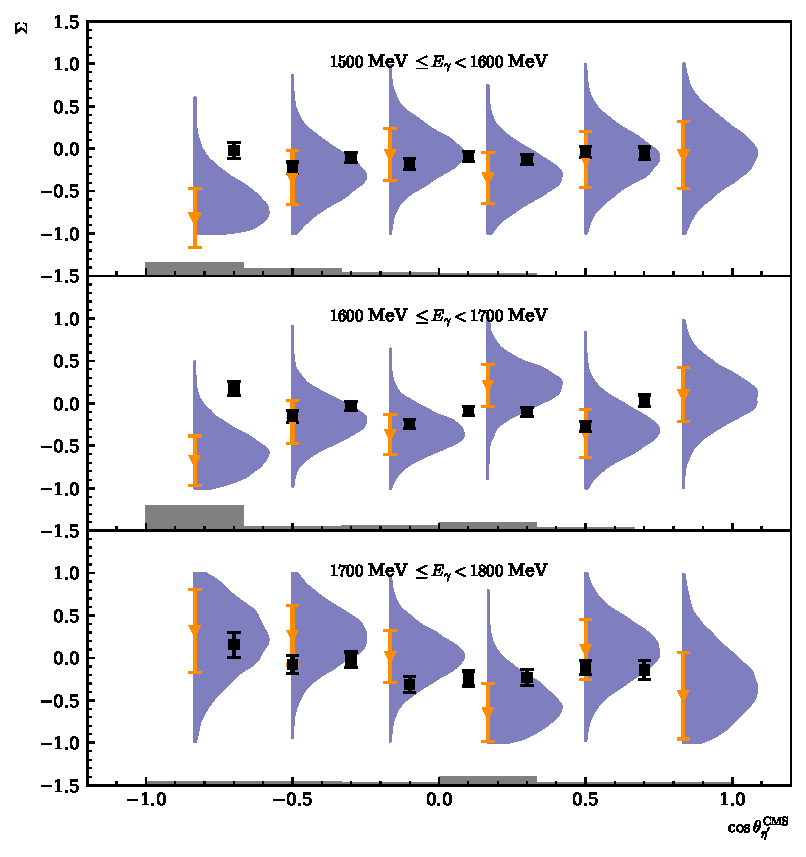
\includegraphics[width=\linewidth]{../bayes/etap_event_based_fit/plots/sigma_etap_data.pdf}
	\caption{Results for the beam asymmetry $\Sigma_{\eta'}$ (orange errorbars and distributions) compared with the results for the energy bins $E_\gamma=\SI{1569}{\mega\eV},E_\gamma=\SI{1676}{\mega\eV},E_\gamma=\SI{1729}{\mega\eV}$ reported in reference \cite{collins} (black errorbars).   Systematical errors are shown as grey bars.}
	\label{fig:etapcollins}
\end{figure}
First of all, one may notice the large difference in statistical errors between the two datasets. This can be explained by considering that the results obtained by \textsc{Collins et al.} \cite{collins} were extracted via the charged decay $\eta'\to\pi^+\pi^-\eta\to2\pi^+2\pi^-\pi^0$ with a branching ratio of $\text{BR}=42.6\cdot22.02\%=9.38\%$ \cite{pdg} as opposed to the neutral decay $\eta'\to\gamma\gamma$ with a branching ratio of $\text{BR}=2.2\%.$ \cite{pdg}. Furthermore, the electrons impinging on the radiator target at CLAS were accelerated to  $\SI{4.5}{\giga\eV}$ \cite{collins}, increasing the statistics in the photon beam energy range of interest compared with CBELSA/TAPS data, where the electrons are only accelerated to  $\SI{3.5}{\giga\eV}$. Aside from the large difference in statistical errors, generally good agreement between the two datasets exists. Most datapoints are compatible within their statistcal errors and the angular profile of the beam asymmetry is displayed equivalently. The largest discrepancy between both datasets exists in backwards direction for the first two energy bins;  although the angular bins do not exactly match it is noteworhty that there is a sign flip between the different measurements that can not be accounted for by combined statistical and systematical error (for the CLAS measurement a systematic error due to the determination of the photon beam polarization of $6\%$ is reported \cite{collins}). It is not understood why these bins show this particular behavior as no indication towards any additional systematic effects has been found. Note however that without identical binning only vague conclusions regarding the agreement of both datasets can be made. The given datasets allow to identify that there is in general consistency and no large unaccounted systematic uncertainties. Direct comparibility can only be achieved if statistics at high center of mass energies are increased. 

Due to the placement of the coherent edge the beam asymmetry $\Sigma_{\eta'}$ could be extracted at beam energies up to $E_\gamma=\SI{1800}{\mega\eV}$ in this work although the CBELSA/TAPS experiment theoretically provides photon beam energies of maximally $E_\gamma^\text{max}=\SI{3200}{\mega\eV}$. Yet, the event yield included less than $10^4$ events collected in roughly four months of beam time. Next to small cross section and branching ratio to a neutral final state this illustrates the effect of Eq. \ref{eq:int} during data collection leading to large statistical errors and background contributions when determining the beam asymmetry. Furthermore only a coarse binning in $\left(E_\gamma,\cos\theta\right)$ could be chosen to account for the available statistics, denying a detailed investigation of the beam asymmetry $\Sigma_{\eta'}\left(E_\gamma,\cos\theta\right)$. In order to collect more statistics at high beam energies in future beam times of the CBELSA/TAPS experiment, e.g. to further investigate the reaction $\gamma p\to p\eta'$, either longer beam times and/or shifting the coherent edge towards higher energies should be considered. Also, the decay channel $\eta'\to\pi^0\pi^0\eta$ may be investigated to increase precision of the existing data.
\section{Comparison of results to PWA calculations}
Figure \ref{fig:pwa} shows the new results for the beam asymmetry $\Sigma$ in $\eta'$ photoproduction obtained with the CBELSA/TAPS experiment compared with existing PWA-predictions. Shown is the etaMAID2018 solution \cite{etaMAID}, which already included results from the measurements \cite{collins} and \cite{thresh} in the fit. This however puts bias towards  the fitted data on the PWA solution such that the same remarks regarding agreement of the results of this thesis and the PWA calculations can be made as in the previous section; generally the obtained data points are described well by the PWA predictions with the exception of the backwards direction at the first two energy bins. This indicates that the previous measurements of $\Sigma_{\eta'}$ had a large influence on the PWA fits, especially when considering that before these measurements were added, the PWA solutions failed to describe the beam asymmetry in $\eta'$ photoproduction, generally showing the wrong sign \cite{collins}. Thus, similarly to the previous section, only a vague conclusion of general agreement between data points and PWA solutions can be drawn.

\begin{figure}[htbp]
\centering
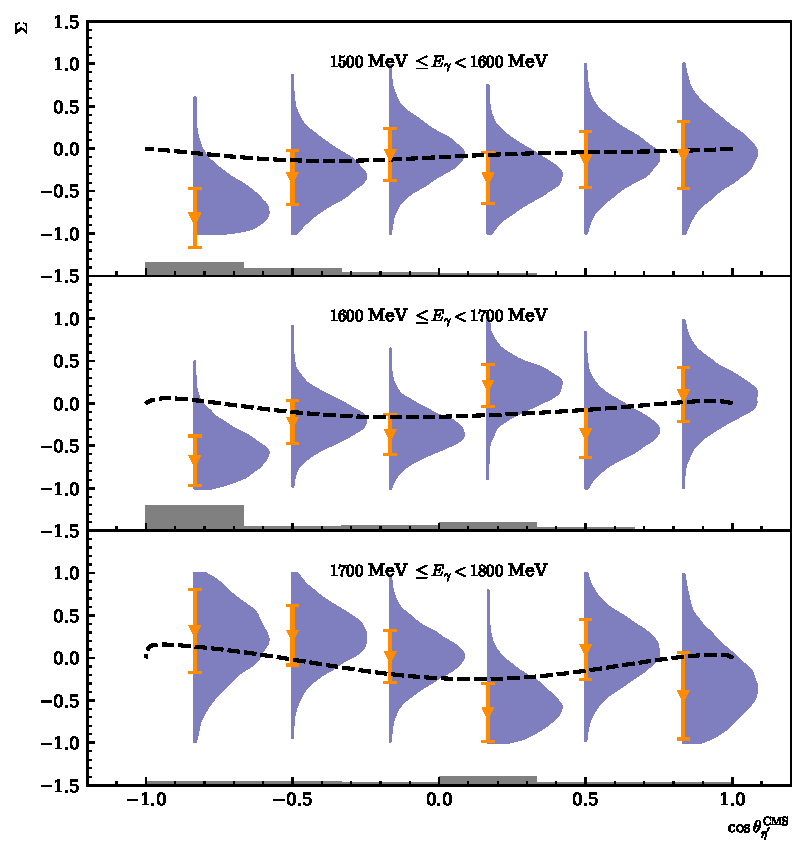
\includegraphics[width=\linewidth]{../bayes/etap_event_based_fit/plots/sigma_etap_pwa.pdf}
\caption{Results for the beam asymmetry $\Sigma_{\eta'}$ (orange errorbars and distributions) compared with PWA solutions:  etaMAID \cite{etaMAID}(dashed black line),\dots The errorbars only depict statistical error, the systematic error is shown as grey bars.}
\label{fig:pwa}
\end{figure}
\section{Final discussion of methods}